% =================================================================
\documentclass[ 10pt, xcolor = dvipsnames]{beamer}
\usepackage{ beamerthemesplit, lmodern}
\usetheme{Madrid}
\usecolortheme[named=Brown]{structure}
\useinnertheme{rectangles}
\setbeamertemplate{frametitle continuation}{}
\beamertemplatenavigationsymbolsempty
\usepackage{../../../macros-general}
\usepackage{../../../macros-beamer}
\AtBeginSection[]
{
\begin{frame}
\frametitle{Contenido del Tema}
\tableofcontents[ currentsection, sectionstyle = show/shaded, subsectionstyle = show/show/hide]
\end{frame}
}
\AtBeginSubsection[]
{
\begin{frame}
\frametitle{Contenido del Tema}
\tableofcontents[ currentsection, currentsubsection, sectionstyle = show/shaded, subsectionstyle = show/shaded/hide]
\end{frame}
}


% =================================================================
\title[Sistemas de Control]{Sistemas de Control (EYAG-1005) }
\author[L. I. Reyes Castro]{Luis I. Reyes Castro}
\institute[ESPOL]{\normalsize Escuela Superior Polit\'ecnica del Litoral (ESPOL) \\ Guayaquil - Ecuador}
\date[2017-T1]{2017 - Primer T\'ermino}

% -----------------------------------------------------------------
\begin{document}
\begin{frame}[noframenumbering]
\titlepage
\end{frame}
\begin{frame}[noframenumbering]
\frametitle{\shorttitle}
\tableofcontents[ subsectionstyle = hide]
\end{frame}


% =================================================================
\section{Sistemas Electromec\'anicos}

% -----------------------------------------------------------------
\begin{frame}[allowframebreaks]
\frametitle{\insertsection}

Modelo del motor DC controlado por armadura: 
\begin{figure}[htb]
\centering
\def\svgwidth{0.9\columnwidth}
\input{motor-dc_armadura.eps_tex}
\end{figure}

\end{frame}

% -----------------------------------------------------------------
\begin{frame}[allowframebreaks]
\frametitle{\insertsection}

\begin{columns}

\begin{column}{0.45\textwidth}
\textbf{Ejemplo \\ (Nise, Problema 2.46*):}
\halfskip

Considere el siguiente mecanismo donde un motor DC controlado por armadura actua sobre un bloque de masa a trav\'es de un sistema de engranajes, donde la entrada es el voltage de entrada del motor $e_a(t)$ y la salida es la posici\'on del bloque de masa $x(t)$. 
\halfskip

Encuentre su funci\'on de transferencia, \iec
\[
G(s) \, = \, \frac{X(s)}{E_a(s)}
\]

\end{column}

\begin{column}{0.45\textwidth}
\begin{figure}[htb]
\centering
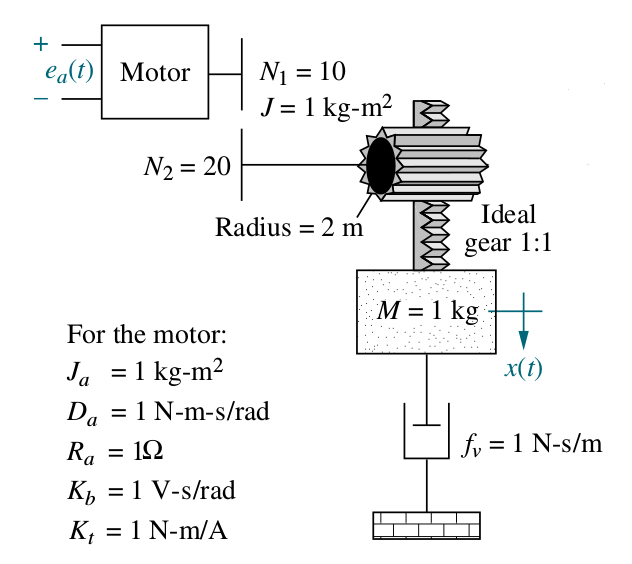
\includegraphics[width=\columnwidth]{nise_prob-2-46.jpeg}
\end{figure}
\fullskip
{
\scriptsize
\textbf{Observaci\'on:} Cada uno de los tres engranajes tiene momento de inercia $J = 1$ kg-m\tsup{2}, mientras que la cremallera es ideal. 
}

\end{column}

\end{columns}
\framebreak

Modelo del motor y del sistema mec\'anico rotacional: 
\begin{figure}[htb]
\centering
\def\svgwidth{0.9\columnwidth}
\input{nise_prob-2-46.eps_tex}
\end{figure}

\end{frame}

% -----------------------------------------------------------------
\begin{frame}[allowframebreaks]
\frametitle{\insertsection}

Modelos: 
\begin{itemize}
\item Motor DC: 
\begin{align*}
T_m(t) \, & = \, K_t \, i_a(t) \\[1ex]
v_a(t) \, & = \, K_b \, \dot{\theta}_1(t) \\[1ex]
e_a(t) \, & = \, R_a \, i_a(t) + v_a(t)
\end{align*}
\item Sistema mec\'anico rotacional: 
\begin{align*}
& J_1 \, \ddot{\theta}_1(t) + J_2 \, \ddot{\theta}_2(t) 
\, = \, T_m(t) - D_a \, \dot{\theta}_1(t) - D_2 \, \dot{\theta}_2(t) \\[1ex]
& N_1 \, \theta_1(t) \, = \, N_2 \, \theta_2(t) \\[1ex]
& x(t) \, = \, r \, \theta_2(t)
\end{align*}
\end{itemize}
\framebreak

Tomando la transformaci\'on de Laplace: 
\begin{itemize}
\item Motor DC: 
\[
E_a(s) \, = \, R_a \, I_a(s) + K_b \, s \, \Theta_1(s)
\]
\item Sistema mec\'anico rotacional: 
\begin{align*}
& ( \, J_1 s^2 + D_a s \, ) \, \Theta_1(s) + 
( \, J_2 s^2 + D_2 s \, ) \, \Theta_2(s) 
\, = \, K_t \, I_a(s) \\[1ex]
& \Theta_1(s) \, = \, ( N_2/N_1 ) \, \Theta_2(s) \\[1ex]
& \Theta_2(s) \, = \, (1/r) \, X(s)
\end{align*}
\end{itemize}
\framebreak

Reemplazando valores para evitar cargar con muchas constantes: 
\begin{itemize}
\item Motor DC: 
\[
E_a(s) \, = \, I_a(s) + s \, \Theta_1(s)
\]
\item Sistema mec\'anico rotacional: 
\begin{align*}
& ( \, 2 s^2 + s \, ) \, \Theta_1(s) + 
( \, 6 s^2 + 2 s \, ) \, \Theta_2(s) 
\, = \, I_a(s) \\[1ex]
& \Theta_1(s) \, = \, 2 \, \Theta_2(s) \, = \, X(s) \\[1ex]
& \Theta_2(s) \, = \, (1/2) \, X(s)
\end{align*}
\end{itemize}
\framebreak

Despejando: 
\begin{itemize}
\item De la ecuaci\'on del motor DC: 
\[
I_a(s) \, = \, E_a(s) - s \, \Theta_1(s)
\]
\item De las ecuaciones del sistema mec\'anico rotacional: 
\begin{align*}
& ( \, 2 s^2 + s \, ) \, \Theta_1(s) + 
( \, 6 s^2 + 2 s \, ) \, \Theta_2(s) \, = \,
E_a(s) - s \, \Theta_1(s) \\[1ex]
\Longrightarrow \quad
& ( \, 2 s^2 + 2 s \, ) \, \Theta_1(s) + 
( \, 6 s^2 + 2 s \, ) \, \Theta_2(s) = \, E_a(s) \\[1ex]
\Longrightarrow \quad
& ( \, 2 s^2 + 2 s \, ) \, X(s) + 
( \, 3 s^2 + s \, ) \, X(s) = \, E_a(s) \\[1ex]
\Longrightarrow \quad
& G(s) \, = \, \frac{1}{ 5 s^2 + 3s }
\end{align*}
\end{itemize}

\end{frame}

% =================================================================
\section{Veh\'iculos Aeroespaciales}

% -----------------------------------------------------------------
\begin{frame}[allowframebreaks]
\frametitle{\insertsection}

Modelos de un ala sencilla con elevador:
\begin{figure}[htb]
\centering
\def\svgwidth{0.9\columnwidth}
\input{simple-wing.eps_tex}
\end{figure}

\end{frame}

% -----------------------------------------------------------------
\begin{frame}[allowframebreaks]
\frametitle{\insertsection}

Aeronave en configuraci\'on Puller (Jalador): 
\begin{figure}[htb]
\centering
\def\svgwidth{\columnwidth}
\input{drone-puller.eps_tex}
\end{figure}

\end{frame}

% -----------------------------------------------------------------
\begin{frame}[allowframebreaks]
\frametitle{\insertsection}

Aeronave en configuraci\'on Pusher (Empujador): 
\begin{figure}[htb]
\centering
\def\svgwidth{\columnwidth}
\input{drone-pusher.eps_tex}
\end{figure}

\end{frame}

\end{document}
